\documentclass[../main]{subfiles}
\begin{document}
\section{Espacios topológicos}\label{part1.1}
        \begin{margintable}\vspace{.8in}\footnotesize
		\begin{tabularx}{\marginparwidth}{|X}
		Section~\ref{part1.1}. Espacios topológicos\\
            Section~\ref{part1.2}. Manifolds \\
            Section~\ref{part1.3}. Espacio tangente\\
            Section~\ref{part1.4}. Formas diferenciales\\
		\end{tabularx}
	\end{margintable}

La noción de manifolds(Variedades diferenciables) es construida en base a los espacios topólogicos.

La noción de TOP. provee conjuntos abiertos y cercados que permiten definir conceptos como continuidad, conectividad y convergencia.

\definicion{(Topologia y espacios topológicos - TOP.) Sea $X$ un conjunto y $\mathcal{T}$ una colección de subconjuntos de $X$ que satisfacen las siguientes propiedades} 

\begin{adjustwidth}{0pt}{-100pt}
\begin{enumerate}
    \item $\emptyset$ y $X$ estan en $\mathcal{T}$
    \item Para una subcolección $\{ u_i \in X \ \backslash \ i \in I\}$, $\bigcup_i u_i \in \mathcal{T}$
    \item Si $u_1, u_2$ $\in X$ entonces $u_1 \cap u_2 \in \mathcal{T}$
\end{enumerate}

Entonces $\mathcal{T}$ es llamado topologia y $(X, Z)$ es llamado espacio topologico.

\textbf{Nota:} Usualmente denotamos $X$ como un espacio TOP. por brevedad. Un elemento de $\mathcal{T}$ es llamado un conjunto abierto.

Sean $(X, \mathcal{T})$ y $(X', \mathcal{T}')$ dos espacios TOP. dado un mapa $f:X\rightarrow X'$, es llamado \textcolor{red}{mapa continuo} si y solo si $f^{-1}(V)\in \mathcal{T}$ para $V \in \mathcal{T}'$.

Si $f$ es biyectivo(inyectivo, sobreyectivo) y ambas $f$ y $f^{-1}$ ($f^{-1}: X'\rightarrow X$) entonces $f$ es llamado \textcolor{red}{Homeomorfismo.}

Sea $(X, \mathcal{T})$ un espacio TOP., entonces un subconjunto de $V$ de $X$ \textcolor{red}{cerrado} si su complemento en $X$ es un conjunto abierto, i.e $X-V \in \mathcal{T}$.

De acuerdo con la definición $X$ y $\emptyset$ son cerrados. Con las siguientes propiedades
\begin{enumerate}[label=(\alph*)]
    \item Para una colección $\{ V_i \ \backslash \ i \in I\}$ de conjuntos cerrados $\cap_i V_i$ es también cerrado.
    \item Para los conjuntos cerrados $V_1, V_2$, $V_1 \cup V_2$ es cerrado.
\end{enumerate}
Una familia $\{ u_i\}$ de conjuntos abiertos de $X$ es llamado un recubrimiento abierto de $X$ si $\bigcup_{i\in I}u_i=X$.

\definicion{Un espacio TOP. es \textcolor{red}{compacto} si cada recubrimiento de $X$ tiene un sub-recubrimiento finito, i.e. si $X=\bigcup_{i\in I}u_i$, para una colección de conjuntos abiertos $\{ u_i\ \backslash \ i\in I\}$, entonces podemos encontrar finitamente muchos $u_{ik}(k=1, \cdots, n)$ tal que $X=\bigcup^n_{k=1}u_{ik}$}

La compacidad es la notación de subconjuntos cerrados y acotados en el espacio euclideano $\mathbb{R}^n$.

\definicion{Un espacio TOP. $X$ es conexo si no puede, ser escrito como $X=X_1 \cup X_2$, donde $X_1$ y $X_2$ son subconjuntos abiertos y $X_1 \cap X_2=\emptyset$. De lo contrario $X$ es llamado disconexos.} 

\definicion{Un espacio topologico es conexo por arcos o arco conexto(path-connected) si, por cada par de puntos $x$ y $x'$ en $X$, hay un camino en $X$ de $x$ a $x'$, hay una función continua $p:[0, 1]\rightarrow X$ tal que $p(0)=x$ y $p(1)=x'$. \\
Todo espacio conexto por arcos es conexo, pero lo contrario no es cierto(¿Algún ejemplo?)}

\definicion{Sea $(X, \mathcal{T})$ un espacio TOP. y $\sim$ es una relación de equivalencia en $X$. Podemos definir una TOP. en el conjunto cociente $X/\sim$ dado por $\mathcal{T}'=\{ u|u \subset X/\sim, p^{-1}(u)\in \mathcal{T}\}$ donde $p:X\rightarrow X/\sim$ es una proyección. Entonces, ($X/\sim, \mathcal{T}')$ es el \textcolor{red}{espacio cociente} de ($X, \mathcal{T}$).}

Supongamos que $\mathcal{T}$ da una topologia a $X$. $N$ es una vecindad de un punto $x\in X$ si $N$ es un subconjunto de $X$ y $N$ contiene algún(al menos uno) conjuntos abierto $u_i$ al que pertenece $x$.

\definicion{Un espacio TOP. se llama \textcolor{red}{espacio de Hausdorff} si por cada $X_1, X_2 \in \mathcal{M}$ de distintos puntos de $X$, existe un vecindario $u_1$, y $u_2$ de $x_1$ y $x_2$ respectivamente, y son disjuntos.\\
En términos generales, dos puntos se pueden ``separar'' en el espacio de Haussdorff. Puede sonar obvio, pero es posible encontrar ejemplos de espacios topológicos que no pueden  ``separar'' dos puntos.}

\textcolor{red}{Recordatorio:} Una función mapea elementos de su dominio a elementos en su codominio. Dada una función $f: X\rightarrow Y$:
\begin{itemize}
    \item 
    \begin{minipage}{0.7\textwidth}
        La función es \textcolor{red}{inyectiva}(uno-a-uno) si cada elemento del codominio se asigna como máxima a un elemetno del dominio, o de manera equivalente, si elementos distintos del dominio se asignan a elementos distintos en el codominio.
        \begin{equation}
            \forall \ x,x' \in X, f(x)=f'(x) \Rightarrow x=x'
        \end{equation}    
    \end{minipage}
    \begin{minipage}{0.5\textwidth}
    \begin{adjustwidth}{0pt}{0pt}
        \begin{center}
            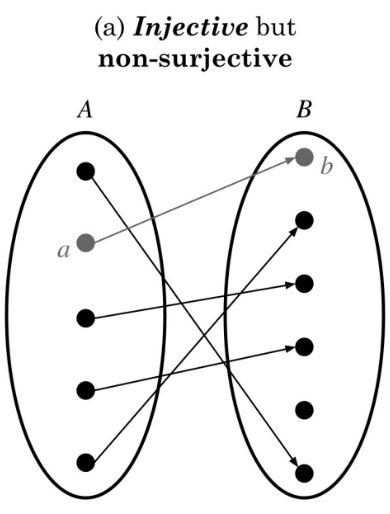
\includegraphics[scale=0.4]{img/inyectiva.PNG}
        \end{center}
    \end{adjustwidth}
    \end{minipage}
    \item 
    \begin{minipage}{0.7\textwidth}
        La función es \textcolor{red}{sobreyectiva}, o sobre, si cada elemento del codominio está mapeado por al menos un elemento del dominio. Es decir, la imagen y el codominio de la función son iguales.
        \begin{equation}
            \forall \ y \in Y, \exists \ x \in X \ \text{tal que} \ y=f(x)
        \end{equation}   
    \end{minipage}
    \begin{minipage}{0.5\textwidth}
    \begin{adjustwidth}{0pt}{0pt}
        \begin{center}
            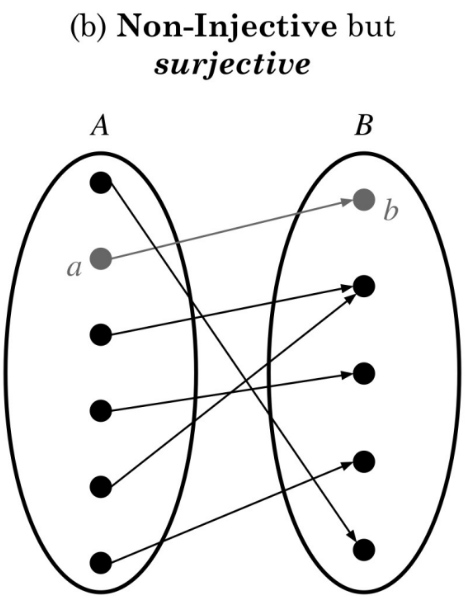
\includegraphics[scale=0.37]{img/sobreyectiva.PNG}
        \end{center}
    \end{adjustwidth}
    \end{minipage}
    \item 
    \begin{minipage}{0.7\textwidth}
        La función es \textcolor{red}{biyectiva}(uno a uno y sobre) si cada elemento del codominio está mapeado por exactamente un elemento del dominio. Es decir, la función es tanto inyectiva como sobreyectiva.
        \begin{equation}
            \forall \ y\in Y, \exists ! \ x\in X \ \text{tal que} \ y=f(x)
        \end{equation}  
    \end{minipage}
    \begin{minipage}{0.5\textwidth}
    \begin{adjustwidth}{0pt}{0pt}
        \begin{center}
            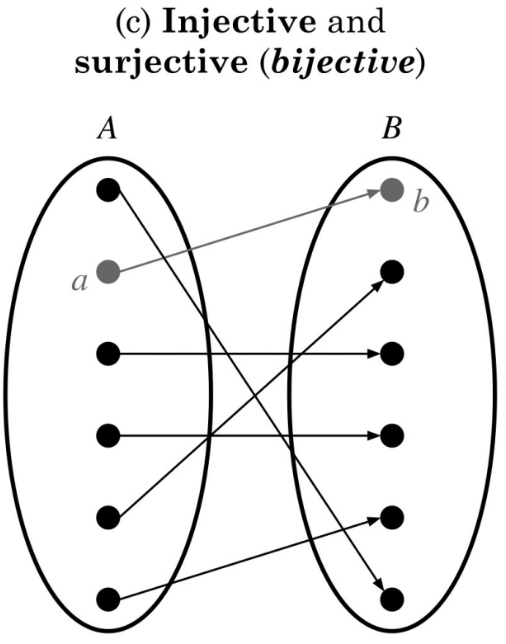
\includegraphics[scale=0.37]{img/biyectiva.PNG}
        \end{center}
    \end{adjustwidth}
    \end{minipage}
\end{itemize}
\section{Manifolds}\label{part1.2}
\definicion{\textcolor{red}{(Manifolds)} Sea $\mathcal{M}$ un espacio de Haussdorff, $\mathcal{M}$ es llamado una manifold suave(diferenciable) n-dimensional si cumple con:}

\begin{enumerate}
    \item Sea $\mathcal{M}=\cup_{\alpha} u_{\alpha}$ de un recubrimiento abierto.
    \item Hay un mapa continuo e invertible
    \begin{equation}
        \varphi_{\alpha}: u_{\alpha} \rightarrow \varphi_{\alpha}(u_{\alpha}) \subseteq \mathbb{R}^n
    \end{equation}
    donde $\varphi(u_{\alpha})$ es abierto en $\mathbb{R}^n$.
    \item Para todo $\alpha, \beta$ tenemos $\varphi(u_{\alpha} \cap u_{\beta})$ es abierto en $\mathbb{R}^n$ y las \textcolor{red}{funciones de transición} serán
    \begin{equation}
        \varphi_{\alpha} \circ \varphi_{\beta}^{-1}: \varphi_{\beta}(u_{\alpha} \cap u_{\beta})\rightarrow \varphi_{\alpha}(u_{\alpha} \cap u_{\beta})
    \end{equation}
    son suaves.
\end{enumerate}

\begin{center}
    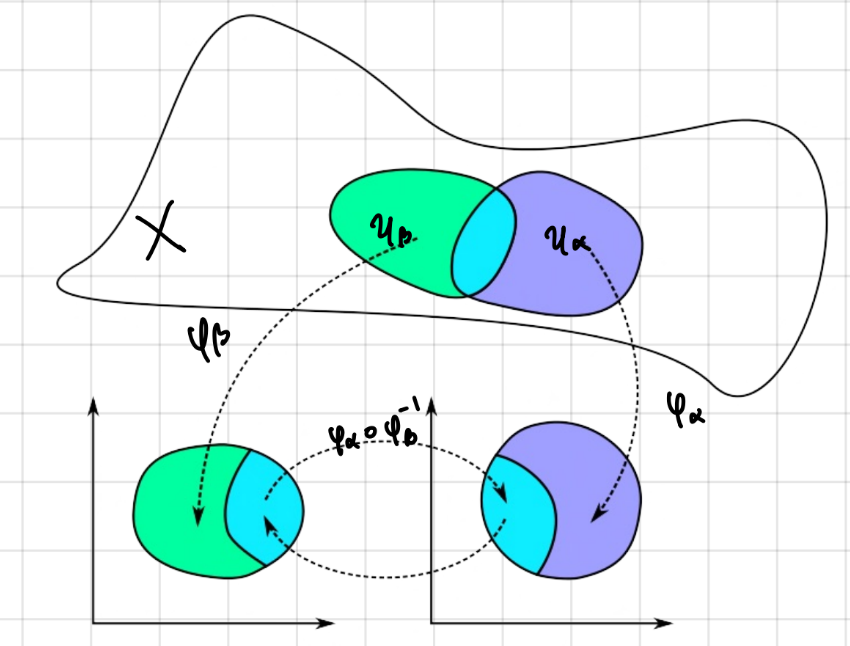
\includegraphics[scale=0.45]{img/imgRG1.PNG}
\end{center}
$(u_{\alpha}, \varphi_{\alpha})$ es llamado un \textcolor{red}{chart de coordenada} y $\{(u_{\alpha}, u_{\alpha})\}_{\alpha}$ es llamado un Atlas. Podemos escribir
\begin{equation}
    \varphi_{\alpha}=(x^1, \cdots, x^n)
\end{equation}
donde cada $x^{i}:u_{\alpha}\rightarrow \mathbb{R}$. Llamamos estos $x^{i}$ \textcolor{red}{coordenadas locales}.

Un punto importante de la definición de una manifold suave es lo siguiente. Si ($u_{\alpha}, \varphi_{\alpha}$) y ($u_{\alpha}, \varphi_{\beta}$) son charts en algún atlas, y $f:\mathcal{M}\rightarrow \mathbb{R}$, entonces $f\circ \varphi^{-1}_{\alpha}$ es suave en $\varphi_{\alpha}(p)$ si y solo si $f\circ \varphi^{-1}_{\beta}$ es suave en $\varphi_{\beta}(p)$ para todo $p\in u_{\alpha} \cap u_{\beta}$.

\ejemplo{Esfera n-dimensional}
Vamos a considerar la esfera n-dimensional
\begin{equation}
    S^n=\{x=(x^0, \cdots, x^n) \in \mathbb{R}^{n+1}: |x|^2=1\}
\end{equation}
Definimos un recubrimiento abierto $\mathcal{M}=S^n=\cup_i u_i$
\begin{align}
    u^{+}=S^n \backslash \{ \text{polo sur}\}, \ u^{-}=S^n \backslash \{ \text{polo norte}\}.
\end{align}
donde el polo norte es $x^0=1$ y el polo sur es $x^0=-1$ y los mapas continuos
\begin{equation}
    \begin{split}
        \varphi^+&: u^+\rightarrow \mathbb{R}^n; \ (x^0, \cdots, x^n) \Rightarrow \dfrac{1}{1+x^0}(x^1, \cdots, x^n)\\
        \varphi^-&: u^-\rightarrow \mathbb{R}^n; \ (x^0, \cdots, x^n) \Rightarrow \dfrac{1}{1-x^0}(x^1, \cdots, x^n)
    \end{split}
\end{equation}
Este mapeo es llamado la proyección estereográfica. Los mapas inversos son
\begin{equation}
    (\varphi^{\pm})^{-1}: \mathbb{R}^n \rightarrow u^{\pm}; (x^1, \cdots, x^n) \Rightarrow \dfrac{1}{1+|x|^2}(\pm(1-|x|^2, 2x^1, \cdots, 2x^n))
\end{equation}
Las funciones de transiciones están dadas por
\begin{equation}
    \varphi^+ \circ (\varphi^-)^{-1}(x)=\dfrac{x}{|x|^2}, \ \varphi^- \circ (\varphi^+)^{-1}(x)=\dfrac{x}{|x|^2}.
\end{equation}

De hecho, la esfera m-dimensional es una manifold compacta.
\begin{center}
    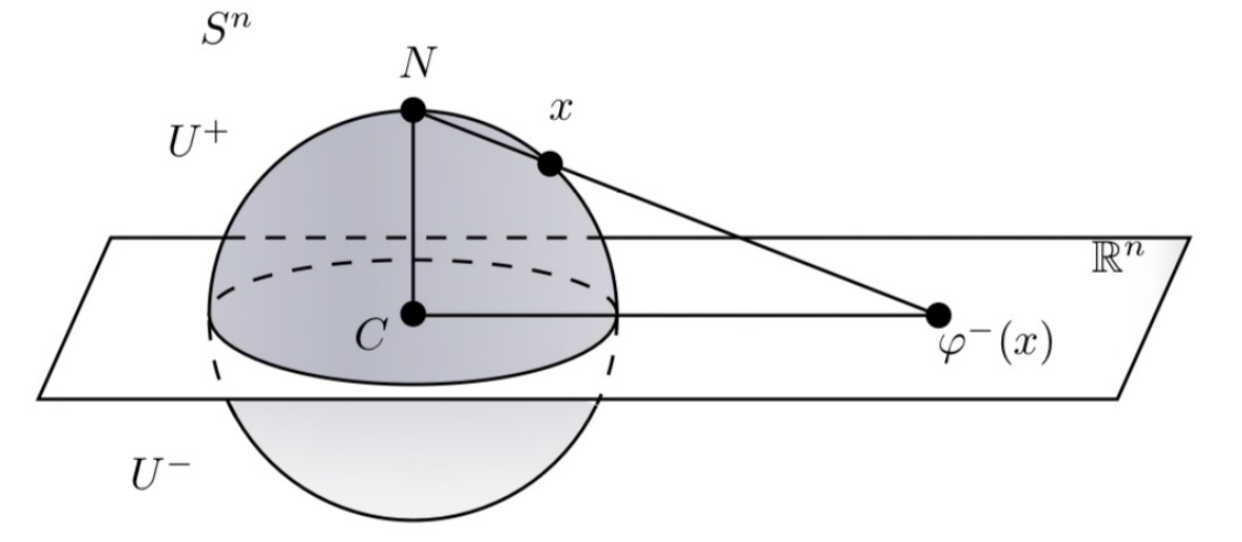
\includegraphics[scale=0.3]{img/imgRG2.PNG}
\end{center}

\definicion{Sea $\mathcal{M}$ una manifold n-dimensional, un subconjunto $\mathcal{M}' \subset \mathcal{M}$ es llamado \textcolor{red}{submanifold}. Si satisface las siguientes propiedad: Para cada $p\in \mathcal{M}'$, existe una coordenada local ($u; x^1, \cdots, x^n$) tal que:}
\begin{equation}
    \mathcal{M}' \cap u=\{ q\in u \Big{|} x^{n'+1}(1)=\cdots x^n(q)=0\}
\end{equation}
De hecho, $\mathcal{M}'$ es n'-dimensional ya que podemos tomar unas coordenadas locales $\mathcal{M}\cap (u; x^1, \cdots, x^n)$ alrededor de $p\in \mathcal{M}'$. Aveces $\mathcal{M}'$ es llamada submanifold de \textcolor{red}{codimensión} $n-n'$ en $\mathcal{M}$. 

\ejemplo{} 
\begin{equation}
    S^n \supset S^{n'}=\{ x=(x^0, \cdots, x^n)\in \mathbb{R}^{n+1}:|x|^2=1, x^{n'+1}=\cdots=x^n=0\}
\end{equation}
es una submanifold de $S^n$.

\definicion{Sea $\mathcal{M}$ y $\mathcal{N}$ manifold con $\dim (\mathcal{M})=m$ y $\dim(\mathcal{N})=n$, entonces tenemos un mapa $f: \mathcal{M}\rightarrow \mathcal{N}$ es \textcolor{red}{suave}, si para un chart $(u_{\alpha}, \varphi_{\alpha})$ de $p \in \mathcal{M}$ y ($V_{\beta}, \psi_{\beta}$) de $f(p) \in \mathcal{N}$, un mapa}
\begin{equation}
    \psi_{\beta}\circ f \circ (\varphi_{\alpha})^{-1}: \varphi_{\alpha}(u_{\alpha} \cap f^{-1}(V_{\beta}))\rightarrow \psi_{\beta}(V_{\beta})
\end{equation}
\textit{es suave. Si, $f$ tiene una inversa suave(en el caso $m=n$), es llamado \textcolor{red}{difeomorfismos}.}

\begin{center}
    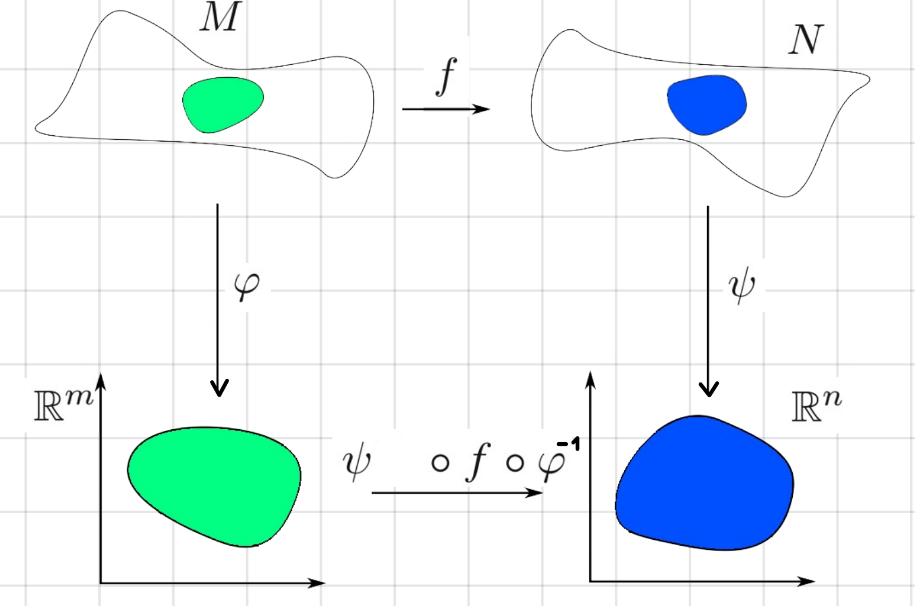
\includegraphics[scale=0.45]{img/imgRG3.PNG}
\end{center}

\textit{Equivalentemente, $f$ es suave en $p$ si $\psi \circ f\circ \varphi^{-1}$ es suave en $\varphi(p)$ para cualquiera de los charts ($u, \varphi$) y ($V, \psi$).}

\ejemplo{}
Sea $\mathcal{M}$ y $\mathcal{N}$ manifolds suaves. Entonces, una proyección $\mathcal{M} \times \mathcal{N} \rightarrow \mathcal{N}$ es un mapa suave.

\ejemplo{}
Una rotación de $S'$ es un difeomorfismo

\section{Espacio tangente}\label{part1.3}
\definicion{(\textbf{Vector tangente}). Un vector tangente $X_p$ en $p\in \mathcal{M}$ es un mapa $X_p:\mathcal{C}^{\infty}(\mathcal{M})\rightarrow \mathbb{R}$, el cual cumple}
\begin{enumerate}
    \item \textcolor{red}{Linearidad:} $X_p(\alpha f+\beta g)=\alpha X_p(f)+\beta X_p(g)$ para $\alpha, \beta \in \mathbb{R}$.
    \item \textcolor{red}{Regla de Leibniz:} $X_p(fg)=f(p)X_p(g)+X_p(f)g(p)$.
\end{enumerate}

Un vector tangente $X_p$ se comporta como una derivada(orden 1) sobre $\mathcal{C}^{\infty}(\mathcal{M})$. Entonces, el conjunto de vectores tangentes en $p$ es un espacio vectorial
\begin{equation}
    (X_p+Y_p)(f)=X_p(f)+Y_p(f),\quad (\alpha X_p)f=\alpha(X_p(f))
\end{equation}
este espacio vectorial es llamado \textcolor{red}{espacio tangente $T_p \mathcal{M}$} en $p\in \mathcal{M}$.

Hay otra forma de pensar en vectores tangentes. Vamos a considerar una curva, la cual es un mapa suave $\gamma:I \rightarrow \mathcal{M}$ con $\gamma(0)=p$ donde $I=(-\epsilon, \epsilon)$ es un intervalo abierto no vacio. 

Dos curvas $\gamma_1, \gamma_2$ son tangentes en $p$ si:
\begin{equation}
    \gamma_1(0)=p=\gamma_2(0),\quad \dv{}{t}\varphi(\gamma_1(t))\Big{|}_{t=0}=\dv{}{t}\varphi(\gamma_2(t))\Big{|}_{t=0}
\end{equation}
\begin{center}
    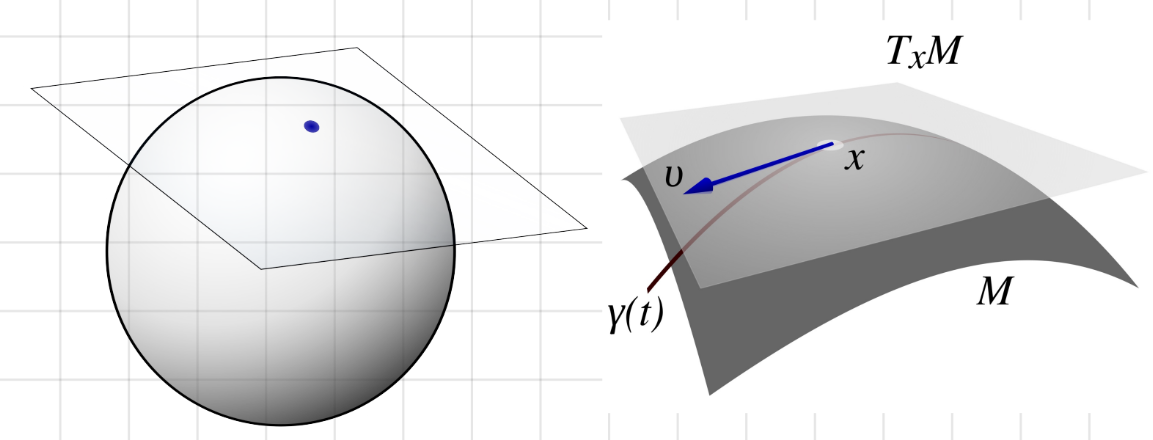
\includegraphics[scale=0.45]{img/imgRG4.PNG}
\end{center}

Donde ($u, \varphi$) es un chart alrededor de $p$. Podemos así escribir dos curvas tangentes $\gamma_1 \sim \gamma_2$, las cuales forman una clase de equivalencia. Para todo $f \in \mathcal{C}^{\infty}(\mathcal{M})$, podemos tomar la derivada de $f$ a lo largo de $\gamma$
\begin{equation}
    X_p(f)=\dv{}{t}\Big{|}_{t=0} f(\gamma(t))
\end{equation}

Es facil ver que $X_p$ satisface la definición de un vector tangente. Así, podemos definir el espacio tangente en $p$
\begin{equation}
    T_p \mathcal{M}=\{\gamma: I\rightarrow \mathcal{M}\ | \ \gamma(0)=p\}/\sim
\end{equation}

Dada unas coordenadas locales $\varphi=(x^1, \cdots, x^n)$, el vector tangente a lo largo de una curva $\gamma$ puede ser escrito como 
\begin{equation}
    X_p=\sum_{i=1}^n X^{i}_p \pdv{}{x^{i}}\Big{|}_p \ \text{donde} \ X^{i}_p=\dv{}{t}X^{i}(\gamma(t))\Big{|}_{t=0}
\end{equation}

Por lo tanto, $\left(\displaystyle \pdv{}{x^1}, \cdots, \pdv{}{x^n}\right)$ puede ser considerado como una base de $T_p\mathcal{M}$.

Supongamos que tenemos también coordenadas $y^1, \cdots, y^n$ cerca de $p$ dado por otro chart. Entonces, podemos escribir 
\begin{equation}
    \pdv{}{y^{i}}\Big{|}_p=\sum_{j=1}^n \pdv{x^j}{y^{i}}(p)\pdv{}{x^j}\Big{|}_p,
\end{equation}
donde $\displaystyle \pdv{x^j}{y^{i}}(p)$ es llamado el \textcolor{red}{Jacobiano} en $p$.

\definicion{Un \textcolor{red}{homomorfismo} es una función $f:\mathbb{R}\rightarrow \mathbb{S}$ la cual satisface las siguientes propiedades:}

\begin{enumerate}
    \item[$i$)] $f(a+b)=f(a)+f(b) \quad \forall \ a,b \in \mathbb{R}$.
    \item[$ii$)] $f(ab)=f(a)f(b)\quad \forall \ a,b \in \mathbb{R}$.
    \item[$iii$)] $f(1_{\mathbb{R}})=1_{\mathbb{S}}$.  
\end{enumerate}
para todo conjunto $\mathbb{R}$ y $\mathbb{S}$.

\definicion{Sea $f: \mathcal{M}^m\rightarrow \mathcal{N}^n$ sea un mapa suave entre dos manifolds. Para $p \in \mathcal{M}$ y cada $v \in T_p \mathcal{M}$, podemos escoger una curva $\gamma:(-\epsilon, \epsilon)\rightarrow \mathcal{M}$ tal que $\gamma(0)=p$ y $\gamma'(0)=v$.\\ \\
El \textcolor{red}{mapa tangente} de $f$ en un punto $p$.}
\begin{equation}
    \mathrm{d}f_p: T_p\mathcal{M}\rightarrow T_{f(p)}\mathcal{N}
\end{equation}
\textit{es definido como} 
\begin{equation}
    (\mathrm{d}f_p)(v)=\beta'(0)
\end{equation}
\textit{donde $\beta=f \circ \gamma:(-\epsilon, \epsilon)\rightarrow \mathcal{N}$.}

\proposicion{} Sea $\mathcal{M}, \mathcal{N}$ y $\mathcal{P}$ manifolds, sea $f: \mathcal{M}\rightarrow \mathcal{N}$ y $g:\mathcal{N}\rightarrow \mathcal{P}$ mapas suaves. Supongamos $q\in \mathcal{M}$, entonces 
\begin{equation}
    \mathrm{d}(g\circ f)=\mathrm{d}g_{f(q)}\circ \mathrm{d}f_q: T_p \mathcal{M}\rightarrow T_{g \circ f(q)} \mathcal{P}.
\end{equation}

\definicion{(\textcolor{red}{Difeomorfismo}). Sea $\mathcal{M}$, $\mathcal{N}$ dos manifolds suaves:}

\begin{enumerate}
    \item[$i$)] Un mapa $f: \mathcal{M}\rightarrow \mathcal{N}$ es llamado \textcolor{red}{difeomorfismo} si $f$ es suave, biyectivo y su mapa inverso $f^{-1}$ es también suave.
    \item[$ii$)] $f: \mathcal{M}\rightarrow \mathcal{N}$ es llamado un \textcolor{red}{difeomorfismo local} en $p \in \mathcal{M}$ si existe un vecindario $U$ de $p$ de $V$ de $f(p)$ tal que $f: U\rightarrow V$ es un difeomorfismo.  
\end{enumerate}

\definicion{(\textcolor{red}{Rango}). Sea $f: \mathcal{M}\rightarrow \mathcal{N}$ un mapa suave. El \textcolor{red}{rango} de $f$ en el punto $p$ es definido como el rango del mapa tangente}
\begin{equation}
    \mathrm{d}f_p: T_p\mathcal{M}\rightarrow T_{f(p)}\mathcal{N}.
\end{equation}

\definicion{(\textcolor{red}{Inmersión, submersión, embeddings y submanifolds}). \\ \\
Sea $f:\mathcal{M}\rightarrow \mathcal{N}$ un mapa suave y $\mathrm{d}f_p: T_p\mathcal{M}\rightarrow T_{f(p)}\mathcal{N}$ el mapa tangente}
\begin{enumerate}
    \item \textit{$f$ es llamada una \textcolor{red}{Inmersión} si $\mathrm{d}f_p$ es inyectivo ($\rank(\mathrm{d} f_p)=\dim \mathcal{M}$) para todo $p\in \mathcal{M}$.}
    \item \textit{$f$ es llamado una \textcolor{red}{Submersión} si $\mathrm{d}f_p$ es sobreyectivo ($\rank(\mathrm{d} f_p)=\dim \mathcal{N}$) para todo $p\in \mathcal{M}$.}
    \item \textit{$f$ es llamado un \textcolor{red}{Embedding} si $f$ es una inmersión y $\varphi: \mathcal{M}\rightarrow \varphi(\mathcal{M})$ es un homeomorfismo.}
    \item \textit{Si $\mathcal{M}\subset \mathcal{N}$ y el mapa de inclusión $i: \mathcal{M}\rightarrow \mathcal{N}$ es un embedding, entonces $\mathcal{M}$ es llamada una \textcolor{red}{submanifold}. de $\mathcal{N}$.}
\end{enumerate}

\boxed{\textcolor{red}{Nota}:}
\begin{enumerate}
    \item Una inmersión no es necesariamente un mapa inyectivo, e.g $f:\mathbb{R} \rightarrow \mathbb{S}^1,\ f(\theta)=e^{i\theta}$.
    \item Una submersión no es necesariamente un mapa sobreyectivo, e.g $f: \mathbb{R} \rightarrow \mathbb{R}, \ f(x)=\arctan(x)$ y $f'(x)=\dfrac{1}{+x^2}$.
\end{enumerate}

\subsection{Bundle Tangentes}
Vamos a considerar la colección de espacios tangente sobre cada punto $p$ sobre $\mathcal{M}$ en una manifold 
\begin{equation}
    T \mathcal{M}=\bigcup_{p \in \mathcal{M}} T_p \mathcal{M}=\{(p, X_p)\Big{|}_p \in \mathcal{M}, X_p \in T_p\mathcal{M}\}
\end{equation}

Existe entonces un mapa natural $\pi: T\mathcal{M}\rightarrow \mathcal{M}$ enviando $X_p \in T_p \mathcal{M}$ a $p$ para cada $p\in \mathcal{M}$ con $\pi$ suave.

Podemos considerar $T\mathcal{M}$ como una manifold de dimensión $2\dim \mathcal{M}$ el cual es llamado el \textcolor{red}{bundle tangente}(fibrado tangente) de $\mathcal{M}$. Sea $x^1, \cdots, x^n$ coordenadas sobre un chart($u, \varphi$). Entonces, para cada $p\in u$ y $X_p \in T_p \mathcal{M}$, hay $\alpha^1, \cdots, \alpha^n \in \mathbb{R}$, tal que:
\begin{equation}
    X_p=\sum_{i=1}^n \alpha^{i} \pdv{}{x^{i}}\Big{|}_p
\end{equation}

Esto da una biyección 
\begin{equation}
    \begin{split}
        \tilde{\varphi}: &\pi^{-1}(u)\rightarrow \varphi(u)\times \mathbb{R}\\
        &X_p \rightarrow (x^1(p), \cdots, x^n(p), \alpha^1, \cdots, \alpha^n)
    \end{split}
\end{equation}

Si $(V, \psi)$ es otro chart sobre $\mathcal{M}$ con coordenadas $y^1, \cdots, y^n$ entonces 
\begin{equation}
    \pdv{}{x^{i}}\Big{|}_p=\sum_{j=1}^n \pdv{y^j}{x^{i}}(p)\pdv{}{y^j}\Big{|}_p,
\end{equation}
de manera que $\tilde{\psi} \circ \tilde{\varphi}^{-1}: \varphi(U \cap V)\times \mathbb{R}^n \rightarrow \psi(U \cap V) \times \mathbb{R}^n$ dado por 
\begin{equation}
    \tilde{\psi}\circ \tilde{\psi}^{-1}(x^1, \cdots, x^n, \alpha^1, \cdots, \alpha^n)=\left(y^1, \cdots, y^n, \sum_{i=1}^n \alpha^{i}\pdv{y^1}{x^{i}}, \cdots, \sum_{i=1}^n \alpha^{i}\pdv{y^n}{x^{i}}\right)
\end{equation}
y es suave.

\subsection{Campos Vectoriales}
Un mapa suave $X: \mathcal{M} \rightarrow T\mathcal{M}$ es llamada \textcolor{red}{sección} de $\pi: T \mathcal{M}\rightarrow \mathcal{M}$ si $\pi X=i\mathrm{d}_M$:
\begin{center}
    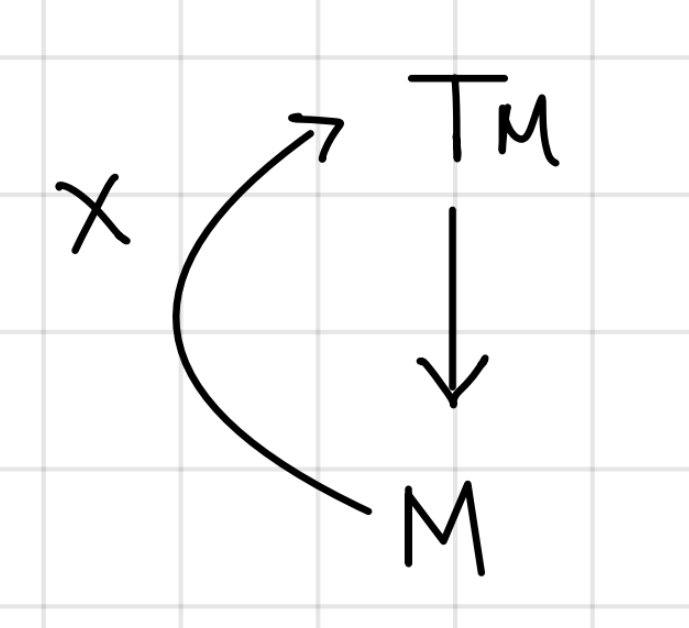
\includegraphics[scale=0.3]{img/imgRG5.PNG}
\end{center}
ya que es una asignación suave $X:p\rightarrow X(p)$, es llamado un \textcolor{red}{campo vectorial}.

\ejemplo{} Sea $\mathbb{S}^n \subset \mathbb{R}^{n+1}$ una n-esfera. Tenemos un campo vectorial $y=\sum y^{i}\pdv{}{x^{i}}$
\begin{equation}
    \text{donde} \ y^{i}=
    \left\{
    \begin{matrix}
        (-x^1, x^0, -x^3, x^2, \cdots, -x^{2k+1}, x^{2k}), \quad n=2k+1\\
        (-x^1, x^0, -x^3, x^2, \cdots, -x^{2k+1}, x^{2k}, 0) \quad n=2k+2.
    \end{matrix}
    \right.
\end{equation}
Podemos escribir un conjunto de campos vectoriales como $\mathfrak{X}(\mathcal{M})=\Gamma (T\mathcal{M})$. De hecho, un campo vectorial $X \in \mathfrak{X}(\mathcal{M})$ es un mapa $\mathcal{C}^{\infty}(\mathcal{M})\rightarrow \mathcal{C}^{\infty}(\mathcal{M})$, el cual satisface:
\begin{enumerate}
    \item[$i$)] $X(\alpha f+\beta g)=\alpha X(f)+\beta X(g)\quad \forall \alpha, \beta \in \mathbb{R}$.\\
    \item[$ii$)] $X(fg)=gX(f)+fX(g)$.  
\end{enumerate}


\begin{center}
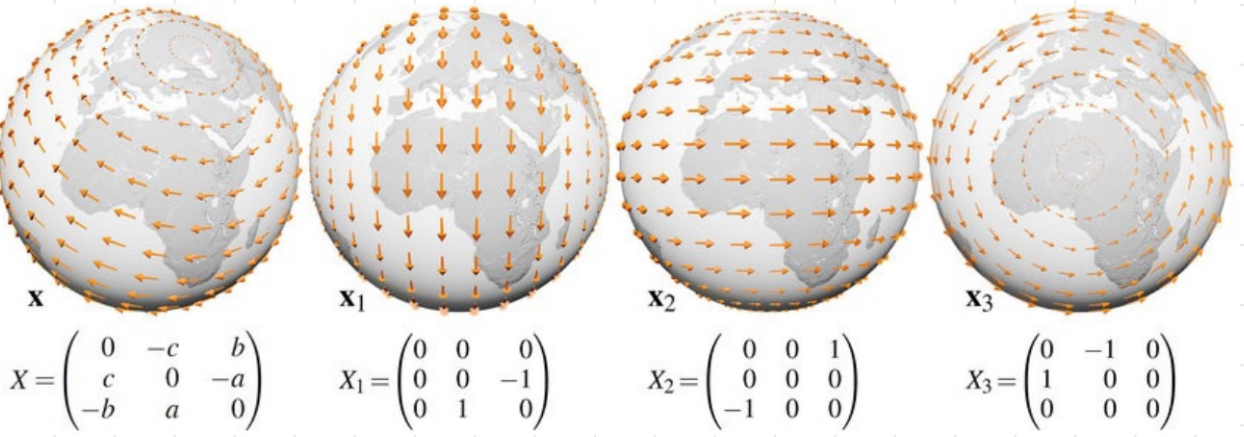
\includegraphics[scale=0.45]{img/imgRG6.PNG}
\end{center}

Sea $X, Y \in \Gamma(\mathcal{M})$ y $f\in C^{\infty}(\mathcal{M})$. Entonces tenemos $X+Y$, $fX \in \Gamma(\mathcal{M})$. Por lo tanto, $\Gamma(\mathcal{M})$ es un $C^{\infty}(\mathcal{M})$ módulo.

Note que el producto de dos campos vectoriales $X, Y \in \Gamma(\mathcal{M})$ no es un campo vectorial:
\begin{equation}
    \begin{split}
        XY(fg)&=X\left(Y(fg)\right)=X\left(fY(g)+gY(f)\right)\\
        &=X(f)Y(g)+fXY(g)+X(g)Y(f)+gXY(f)
    \end{split}
\end{equation}

Sin embargo, $XY-YX$ es un capo vectorial denotado como $[X, Y]$ es llamado el \textcolor{red}{bracket de Lie}. De hecho, $\Gamma(\mathcal{M})$ con brackets de Lie satisface:
\begin{enumerate}
    \item[$i$)]  $[\cdot, \cdot]$ es bilineal.
    \item[$ii$)] $[\cdot, \cdot]$ es antisimetrico, i.e $[X, Y]=-[Y, X]$.
    \item[$iii$)] La \textcolor{red}{identidad de Jacobi} se cumple 
    \begin{equation*}
        \left[X, [Y, Z]\right]+\left[Y, [Z, X]\right]+\left[Z, [X, Y]\right]=0
    \end{equation*}
\end{enumerate}

\subsection{Flujo}
Una \textcolor{red}{curva integral} de un campo vectorial $X \in \Gamma(\mathcal{M})$ es un mapa suave $\gamma: I\rightarrow \mathcal{M}$ tal que $I$ es un intervalo abierto en $\mathbb{R}$ y $\dot{\gamma}(t)=X_{\gamma}(t)$.

\ejemplo{} Un campo vectorial $\displaystyle X=\alpha \pdv{}{x}+\beta \pdv{}{y}$ en $\mathbb{R}^2$. Entonces la curva integral es una traslación
\begin{equation}
    \gamma_t(x, y)=(x+t\alpha, y+t\beta).
\end{equation}

Supongamos que un campo vectorial puede ser escrito en terminos de unas coordenadas locales $(x^1, \cdots, x^n)$ sobre un vecindario abierto $u$ alrededor de $p \in \mathcal{M}$.
\begin{equation}
    X=\sum_{i=1}^n \alpha^{i} \pdv{}{x^{i}}
\end{equation}

Entonces $\dot{\gamma}(t)$ se puede expresar $\displaystyle \dot{\gamma}(t)=\dv{x^{i}}{t}=\alpha^{i}(x^1(t), \cdots, x^n(t))$.

Estas son simplemente ecuaciones diferenciales y $\gamma(t)$ es una curva integral. Además, existe un teorema que establece que existe una única solución $\gamma:(-\epsilon, \epsilon) \rightarrow \mathcal{M}$ para un $\epsilon>0$ suficientemente pequeño tal que $\gamma(0)=p$.

\teorema{(Existencia de curvas integrales).} Sea $X \in \Gamma(\mathcal{M})$ y $p \in \mathcal{M}$. Entonces, existe un intervalo abierto $I \subseteq \mathbb{R}$ con $0 \in I$ y una curva integral $\gamma: I \rightarrow \mathcal{M}$ para $X$ con $\gamma(0)=p$. Además, si $\tilde{\gamma}: \tilde{I} \rightarrow \mathcal{M}$ es otra curva integral para $X, Y$ $\tilde{\gamma}(0)=p$, entonces $\tilde{\gamma}=\gamma$ en $I \cap \tilde{I}$.

Si $\gamma(t)$ es definido para cualquier $t \in \mathbb{R}$ sobre $\mathcal{M}$, entonces $X$ es llamado \textcolor{red}{completo}. Si $\mathcal{M}$ es una manifold suave y compacta, cualquier campo vectorial es completo. En esta situación, un mapa suave 
\begin{equation}
    \begin{split}
        \gamma:&\mathbb{R} \times \mathcal{M} \rightarrow \mathcal{M}; \\
        &(t, p) \rightarrow \gamma_t(p)
    \end{split}
\end{equation}
es llamado \textcolor{red}{flujo}(o grupo de un parámetro de difeomorfismo) generado por un vector $X$ el cual satisface 
\begin{equation}
    \gamma_{t+s}(p)=\gamma_t(\gamma_s(p))=\dv{\gamma_t(p)}{t}=X_{\gamma_t(p)}
\end{equation}

\section{Formas Diferenciales}\label{part1.4}
\subsection{Bundles Cotangentes}
Dado un espacio vectorial $V$ en $\mathbb{R}$, podemos tomar su campo dual 
\begin{equation}
    V^{*}=\{w: V\rightarrow \mathbb{R}\ | \ w(\alpha_1 X_1+\alpha_2 X_2)=\alpha_1 w(X_1)+\alpha_2 w(X_2) \ \text{para} \ X_i \in V \ \text{y} \ \alpha_i \in \mathbb{R}\}
\end{equation}

El espacio dual $V^{*}$ es también un espacio vectorial $\beta_1 w_1+\beta_2 w_2 \in V^{*}$ para $w_1, w_2 \in V^{*}$ y $\beta_1, \beta_2 \in \mathbb{R}$. El espacio vectorial dual $T^{*}_p \mathcal{M}$ del espacio tangente $T_p \mathcal{M}$ es llamado el \textcolor{red}{espacio cotangente}.

De hecho, dado $f \in C^{\infty}(\mathcal{M})$, podemos definir su diferencial $\mathrm{d}f_p$ en $p$:
\begin{equation}
    \begin{split}
        \mathrm{d}f_p:& T_p \mathcal{M} \rightarrow \mathbb{R},\\
        & X_p \rightarrow X_p(f).
    \end{split}
\end{equation}

Para unas coordenadas locales $(u, \varphi=(x^1, \cdots, x^n))$, hemos visto que $\displaystyle \left(\pdv{}{x^1}\Big{|}_p, \cdots, \pdv{}{x^n}\Big{|}_p\right)$ es una base de $T_p\mathcal{M}$.

Por otra parte, podemos tomar $\left(\mathrm{d}x^1\Big{|}_p, \cdots, \mathrm{d}x^n\Big{|}_p\right)$ como una base de $T^{*}_p \mathcal{M}$, tal que: 
\begin{equation}
    \mathrm{d}x^j\Big{|}_p \left(\pdv{}{x^{i}}\Big{|}_p\right)=\delta^j_i.
\end{equation}

Por lo tanto, en esta base, podemos escribir $\displaystyle\mathrm{d}f_p=\sum_{i=1}^n \pdv{f(p)}{x^{i}}\mathrm{d}x^{i}\Big{|}_p$.

Al igual que el bundle tangente, podemos considerar una colección de espacios cotangentes:
\begin{equation}
    T^{*}\mathcal{M}=\bigcup_{p \in \mathcal{M}} T^{*}_p \mathcal{M}
\end{equation}

La cual posee estructura de una manifold. Llamamos $T^{*}\mathcal{M}$ el \textcolor{red}{bundle cotangente} de $\mathcal{M}$. Además, la sección del espacio cotangente es llamado 1-forma, y denotamos el conjunto de 1-forma por $\Omega^1(\mathcal{M})=\Gamma(T^{*}\mathcal{M})$.
\vspace{1cm}
\hrule

\begin{minipage}[t]{0.5\textwidth}
\begin{adjustwidth}{0pt}{20pt}
    \centerline{\textcolor{red}{Bundle tangente}}
    \begin{equation*}
        TM=\bigcup_p T_p \mathcal{M}
    \end{equation*}
    \vspace{-0.7cm}
    \begin{align*}
        \pi&: T\mathcal{M} \rightarrow \mathcal{M} \\
        \pi^{-1}&: \mathcal{M} \rightarrow T\mathcal{M}
    \end{align*}
    \vspace{-0.9cm}
    \begin{align*}
        \pi^{-1}: \Gamma(T\mathcal{M})=\mathfrak{X}(\mathcal{M})
    \end{align*}
    \vspace{-0.9cm}
    \begin{align*}
         \mathfrak{X}(\mathcal{M}): &\text{Espacio donde viven}\\
         &\text{los vectores}\\
         &\rightarrow X \in \mathfrak{X}(\mathcal{M})
    \end{align*}
    Sea $X^1, \cdots, X^n$ coordenadas sobre un chart $(u, \varphi)$. Entonces, para cada $p \in u$ y $X \in \mathfrak{X}(\mathcal{M})$ hay $\alpha^1, \cdots, \alpha^n \in \mathbb{R}$ tal que:
    \begin{equation*}
        X_p=\sum_{i=1}^n \alpha^{i}\pdv{}{x^{i}}\Big{|}_p
    \end{equation*}
\end{adjustwidth}
\end{minipage}
    \hspace{0.01\textwidth} % Espacio entre las dos minipages
    \vrule % Línea vertical
    \hspace{0.01\textwidth} % Espacio entre las dos minipages
\begin{minipage}[t]{0.5\textwidth}
\begin{adjustwidth}{20pt}{0pt}
    \centerline{\textcolor{red}{Bundle cotangente}}
    \begin{equation*}
        T^{*}\mathcal{M}=\bigcup_p T^{*}_p \mathcal{M}
    \end{equation*}
    \vspace{-0.7cm}
    \begin{align*}
        \pi^{*}&: T^{*}\mathcal{M} \rightarrow \mathcal{M} \\
        \pi^{*^{-1}}&: \mathcal{M} \rightarrow T^{*}\mathcal{M}
    \end{align*}
    \vspace{-0.9cm}
    \begin{align*}
        \pi^{*^{-1}}: \Gamma(T^{*}\mathcal{M})=\Omega^1(\mathcal{M})
    \end{align*}
    \vspace{-0.9cm}
    \begin{align*}
         \Omega^1(\mathcal{M}): &\text{Espacio donde viven}\\
         &\text{las 1-formas}\\
         &\rightarrow w \in \Omega^1(\mathcal{M})
    \end{align*}
    Sea $X^1, \cdots, X^n$ coordenadas sobre un chart $(u, \varphi)$. Entonces, para cada $p \in u$ y $w \in \Omega^1(\mathcal{M})$, hay $\beta^1, \cdots, \beta^n \in \mathbb{R}$ tal que:
    \begin{equation*}
        w_p=\sum_{i=1}^n \beta_1 \mathrm{d}x^{i}\Big{|}_p
    \end{equation*}
\end{adjustwidth}
\end{minipage}

Tal que:
\begin{align*}
    \ w: &X \rightarrow \mathbb{R} \\
    &X \rightarrow w(X) \in \mathbb{R}
\end{align*}
y localmente $\mathrm{d}x^{j}\Big{|}_p \left(\pdv{}{x^{i}}\Big{|}_p\right)=\delta^j_i$.

\ejemplo{} Si $f$ es una función suave sobre $\mathcal{M}$, entonces $\mathrm{d}f \in \Omega^1(\mathcal{M})$, el cual podemos emparejar con $\forall X \in \mathfrak{X}(\mathcal{M}): \mathrm{d}f(X)=X(f) \in \mathbb{R}$.

\subsection{Push-forward y Pull-back}
Sea $f: \mathcal{M}\rightarrow \mathcal{N}$ un mapa suave entre las manifolds $\mathcal{M}$ y $\mathcal{N}$, $f$ induce un \textcolor{red}{push-forward} de vectores tangentes
\begin{equation}
    f_{*}: T_p \mathcal{M} \rightarrow T_{f(p)}\mathcal{N}
\end{equation}

El cual es definido por $f_{*}(X_p)(g)=X_p(g \circ f)$ para $g \in C^{\infty}(\mathcal{M})$. $f_*$ es denotada por $\mathrm{d}f_p$ en la literatura.
\begin{center}
    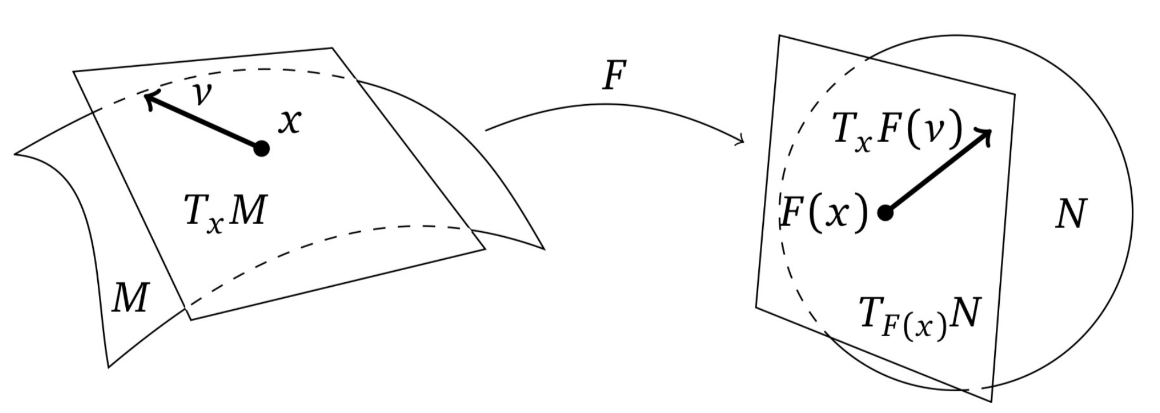
\includegraphics[scale=0.4]{img/imgRG7.PNG}
\end{center}

Por otra parte, $f$ induce un \textcolor{red}{pull-back} del espacio tangente $f^{*}: T^{*}_{f(p)}\mathcal{N} \rightarrow T^{*}_p \mathcal{M}$ el cual es definido por 
\begin{equation}
    \langle f^*(w_{f(p)}, X_p)\rangle = \langle w_{f(p)}, f_*(X_p)\rangle
\end{equation}
para $w_{f(p)} \in T_{f(p)}\mathcal{N}$ donde $\langle \cdot, \cdot \rangle$ es un emparejamiento entre el espacio tangente y espacio cotangente.

Si $f_*: T_p \mathcal{M}\rightarrow T_{f(p)}\mathcal{N}$ es suryectivo, i.e $\rank(f_*)=\dim \mathcal{N}$, entonces $f$ es \textcolor{red}{regular} en el punto $p \in \mathcal{M}$. De lo contrario, $p \in \mathcal{M}$ es llamado un \textcolor{red}{punto crítico} de $f$ y $f(p) \in \mathcal{N}$ es llamado el \textcolor{red}{valor crítico} de $f$.

\ejemplo{} Sea $f: \mathbb{S} \rightarrow \mathbb{R}$ sea un mapa definido por $f(x^1, \cdots, x^n)=x^n$ donde $\mathbb{S}^n=\{(x^0, \cdots, x^n) \in \mathbb{R}^{n+1} \ | \ |x|=1\}$. Entonces, el polo norte y polo sur $x^n=\pm 1$ son puntos críticos de $f$ y un punto genérico es regular. 

\definicion{Si $f_*$ es regular para $\forall p \in \mathcal{M}$, $f$ es llamado una \textcolor{red}{submersión}. Para $q \in f(\mathcal{M})$, $f^{-1}(q)$ es una submanifold de codimensión $\dim(\mathcal{N})$ en $\mathcal{N}$.}

\ejemplo{} La proyección $f: \mathcal{M} \times \mathcal{N} \rightarrow \mathcal{M}$ es una submersión.

\subsection{Cambio de coordenadas}
Supongamos que $(U, \varphi)$ y $(V, \psi)$ son dos chart suaves sobre $\mathcal{M}$, y $p \in U\cap V$. Vamos a denotar una función coordenada $\varphi$ por $(x^{i})$ y para $\psi$ por $(\tilde{x}^{i})$.

Cualquier vector tangente en $p$ puede ser representado con respecto a cualquiera de las bases $\displaystyle \left(\pdv{}{x^{i}}\Big{|}_p\right)$ o $\displaystyle \left(\pdv{}{\tilde{x}^{i}}\Big{|}_p\right)$. ¿Cómo pueden estar relacionadas estas representaciones?

Podemos escribir los mapas de transición $\psi \circ \varphi^{-1}(x)=\left(\tilde{x}^{i}(x), \cdots, \tilde{x}^{n}(x)\right)$ mediante el push-forward por $\psi \circ \varphi^{-1}$ podemos escribir 
\begin{equation}
    (\psi \circ \varphi^{-1}) *\pdv{}{x^{i}}\Big{|}_{\varphi(p)}=\pdv{\tilde{x}^{j}}{x^{i}}(\varphi(p))\pdv{}{\tilde{x}^{j}}\Big{|}_{\psi(p)}
\end{equation}

Entonces, obtenemos 
\begin{equation}
    \begin{split}
        \pdv{}{x^{i}}\Big{|}_p&=(\varphi^{-1}) * \pdv{}{x^{i}}\Big{|}_{\varphi(p)}=(\psi^{-1})*(\psi \circ \varphi^{-1})*\pdv{}{x^{i}}\Big{|}_{\varphi(p)}=(\psi^{-1})*\pdv{\tilde{x}^{j}}{x^{i}}(\varphi(p))\pdv{}{\tilde{x}^j}\Big{|}_{\psi(p)}\\
        &=\pdv{\tilde{x}^j}{x^{i}}(\varphi(p))(\psi^{-1})*\pdv{}{\tilde{x}^j}\Big{|}_{\varphi(p)}=\pdv{\tilde{x}^j}{x^{i}}(\varphi(p))\pdv{}{\tilde{x}^j}\Big{|}_p,
    \end{split}
\end{equation}
donde $\varphi(p)$ es la representación de coordenadas de $p$ en $x^{i}$-coordenadas. Aplicando lo anterior a las componentes de un vector $\displaystyle x=x^{i}\pdv{}{x^{i}}\Big{|}_p=\tilde{x}^j\pdv{}{\tilde{x}^j}\Big{|}_p$, encontramos que las componentes transforman(mediante la regla de cadena)
\begin{equation}
    \tilde{X}^j=\pdv{\tilde{X}^j}{x^{i}}(\varphi(p))X^{i}.
\end{equation}

Una manifold suave $\mathcal{M}$ es \textcolor{red}{orientable} si y solo si existe un atlas $\{ (u_{\alpha}, \varphi_{\alpha})\}$ de $\mathcal{M}$ tal que el determinante del Jacobiano es positivo en cualquier $U_{\alpha} \cap U_{\beta}$.


\subsection{Formas diferenciales}
Es natural considerar un álgebra generada por la base de $T^{*}_p \mathcal{M}$ sobre $\mathbb{R}$ que satisface 
\begin{equation}
    \mathrm{d}x^{i} \wedge \mathrm{d}x^j=-\mathrm{d}x^j \wedge \mathrm{d}x^{i}
\end{equation}
donde $\wedge$ es llamado el producto Wedge, puede ser entendido como una multiplicación de esta álgebra, y llamamos $\wedge$ el \textcolor{red}{álgebra exterior}. Para una manifold n-dimensional, tenemos una descomposición de sumas directas
\begin{equation}
    \wedge^{*}T^{*}_p \mathcal{M}=\bigoplus_{k=0}^n \wedge^k T^{*}_p \mathcal{M}.
\end{equation}

Un elemento $w \in \wedge^* T^*_p \mathcal{M}$ define un mapa k-linear alternante $T_p \mathcal{M} \times \cdots \times T_p \mathcal{M} \rightarrow \mathbb{R}$ con 
\begin{equation}
    w(X_{\sigma(1)} \cdots X_{\sigma(k)})=\sign(\sigma) w(X_1, \cdots, X_k),\quad (X_i \in V)
\end{equation}

Para $\sigma \in \mathcal{S}_k$. Además, para un elemento $w=w_1\wedge w_2\wedge \cdots \wedge w_k$, definimos:
\begin{equation}
    w_1\wedge w_2\wedge \cdots \wedge w_k(X_1, X_2, \cdots, X_k)=\dfrac{1}{k!}\det(w_a(X_b))
\end{equation}

Generalmente, si $w$ es una k-forma y $\eta$ es una 1-forma 
\begin{equation}
    (w \wedge \eta)(X_1, \cdots, X_{k+1})=\dfrac{1}{(k+l)!}\sum_{\sigma \in \mathcal{S}_{k+1}} \sign(\sigma) w(X_{\sigma(1)}, \cdots, X_{\sigma(\alpha)})\eta(X_{\sigma(k+1)}, \cdots, X_{\sigma(k+l)})
\end{equation}

Podemos considerar una familia de espacios vectoriales sobre la manifold $\mathcal{M}$. $\wedge^k T^* \mathcal{M}=\bigcup_p \wedge^k T^*_p \mathcal{M}$ la cual satisface la definición 7 de una manifold.  Dado dos coordenadas locales $(u, x^1, \cdots, x^n)$ y $(v, y^1, \cdots, y^n)$, la transformación es dada por 
\begin{equation}
    \mathrm{d}x^{i1}\wedge \cdots \wedge \mathrm{d}x^{ik}=\sum_{j_1 < \cdots <j_k} \pdv{D(x^{i1}, \cdots, x^{ik})}{D(y^{j1}, \cdots, y^{jk})} \mathrm{d}y^{j1} \wedge \cdots \wedge \mathrm{d}y^{jk}
\end{equation}
donde $\displaystyle \dfrac{D(\cdots)}{D(\cdots)}$ denota el Jacobiano. Además, escribimos el conjunto de todas las secciones como 
\begin{equation}
    \Omega^k(\mathcal{M})=\Gamma(\wedge^* T^* \mathcal{M}).
\end{equation}

En particular, tenemos $\Omega^0(\mathcal{M})=C^{\infty}(\mathcal{M})$. Un elemento de $\Omega^k(\mathcal{M})$ es conocido como una \textcolor{red}{k-forma diferencial}. Como resultado, una k-forma puede ser expresado como 
\begin{equation}
    \begin{split}
        w&=\sum_{i_1<\cdots <i_k}f_{i_1\cdots i_{\alpha}}(x^1, \cdots, x^n)\mathrm{d}x^{i_1}\wedge \cdots \wedge \mathrm{d}x^{i_{\alpha}}
    \end{split}
\end{equation}

En la intercepción de dos charts locales $(u; x^1, \cdots, x^n)$ y $(v; y^1, \cdots, y^n)$, y $f, g$ están relacionadas por el Jacobiano. Poniendo todos los $p$ juntos, un elemento $w \in \Omega^k(\mathcal{M})$ define un mapa alternante k-lineal 
\begin{equation}
    w: \mathfrak{X}(\mathcal{M})\times \cdots \times \mathfrak{X}(\mathcal{M}) \rightarrow C^{\infty}(\mathcal{M}).
\end{equation} 

Además, existe un mapa lineal único llamado la \textcolor{red}{derivada exterior} $\mathrm{d}: \Omega^k(\mathcal{M})\rightarrow \Omega^{k+1}(\mathcal{M})$ tal que:
\begin{enumerate}
    \item[($i$)] En $\Omega^0(\mathcal{M})$, esto fue ya definido, i.e $\mathrm{d}f=X(f)$ para todo $X\in \mathfrak{X}(\mathcal{M})$.
    \item[($ii$)] Tenemos $\mathrm{d} \circ \mathrm{d}=0: \Omega^k(\mathcal{M})\rightarrow \Omega^{k+2}(\mathcal{M})$.
    \item[($iii$)] Satisface la \textcolor{red}{regla de Leibniz} $\mathrm{d}(w \wedge \eta)=\mathrm{d}w \wedge \eta+(-1)^k w \wedge \mathrm{d}\eta$. 
\end{enumerate}
Para $w \in \Omega^k(\mathcal{M})$, la derivada exterior puede ser definida como 
\begin{equation}
    \begin{split}
        (\mathrm{d}w)(X_1, \cdots, X_{k+1})&=\dfrac{1}{k+1}\left\{\sum_{i=1}^{k+1} (-1)^{i+1} X_i\left(w(X_1, \cdots, \hat{X}_i, \cdots, X_{k+1})\right)\right.\\
        &\quad +\left.\sum_{i<j}(-1)^{i+j}w\left([X_i, X_j], X_1, \cdots, \hat{X}_i, \cdots, \hat{X}_j, \cdots, X_{k+1}\right)\right\}
    \end{split}
\end{equation}
donde $\forall X_1, \cdots, X_{k+1} \in \mathfrak{X}(\mathcal{M})$ y $\wedge$ significa omitido.

En términos de coordenadas locales $x^1, \cdots, x^n$, podemos definir las derivadas exteriores como 
\begin{equation}
    \mathrm{d}\left(\sum_{i_1<\cdots<i_k} w_{i_1, \cdots, i_k}\mathrm{d}x^{i_1}\wedge\cdots \wedge \mathrm{d}x^{ik}\right)=\sum \mathrm{d}w_{i_1, \cdots, i_k}\wedge \mathrm{d}x^{i_1}\wedge \cdots \wedge \mathrm{d}x^{ik}
\end{equation}

Sea $f: \mathcal{M}\rightarrow \mathcal{N}$ un mapa entre manifolds suaves $\mathcal{M}$ y $\mathcal{N}$. Esto induce un homomorfismo de álgebra 
\begin{equation}
    f^*: \Omega^{\bullet}(\mathcal{N})\rightarrow \Omega^{\bullet}(\mathcal{M})
\end{equation}

El pull-back de formas diferenciales asociado a $f$ puede ser definido como 
\begin{equation}
    (f^* w)(X_1, \cdots, X_k)=w\left(f_*(X_1), \cdots, f_*(X_k)\right).
\end{equation}

Para $\omega \in \Omega^k(\mathcal{N})$ y $X_1, \cdots, X_n \in \mathfrak{X}(\mathcal{M})$. Note que el pull-back $f^*$ tiene las siguientes propiedades:
\begin{enumerate}
    \item[$(i)$] $f^*: \Omega^k(\mathcal{N}) \rightarrow \Omega^k(\mathcal{M})$ es un mapa linear.
    \item[$(ii)$] $f^*(\omega \wedge \eta)=f^* \omega \wedge f^* \eta$.
    \item[$(iii)$] Si $g: \mathcal{N}\rightarrow \mathcal{L}$ es un mapa entre dos manifolds $\mathcal{N}$ y $\mathcal{L}$, entonces $(g \circ f)^*=f^* \circ g^*$.
    \item[$(iv)$] Conmmuta con derivada exterior $\mathrm{d}f^*=f^* \mathrm{d}$. 
\end{enumerate}

\definicion{\textcolor{red}{(Co-Vector)}}. Un Covector es un mapa linear desde un espacio vectorial a $\mathbb{R}$.
\begin{equation}
    \omega: \mathbb{V} \rightarrow \mathbb{R}, \quad \omega(V)\in \mathbb{R}
\end{equation}
el co-vector $\omega$ es definido en el espacio vectorial dual $\mathbb{V}^*$.

Ahora, veremos que el espacio dual al espacio tangente $T_p(\mathcal{M})$, el cual llamamos $T^*_p(\mathcal{M})$.

Sea $f:\mathcal{M}\rightarrow \mathbb{R}$ una función suave, definimos un co-vector $\mathrm{d}f$ por:
\begin{equation}
    \mathrm{d}f(V):=V(f) \quad \text{con} \quad V\in T_p(\mathcal{M}).
\end{equation}

Si $V=\partial_{\mu}$(bases coordenadas de un vector) y $f=x^{\mu}$(funciones coordenadas)
\begin{equation}
    \mathrm{d}x^{\mu}(\partial_{\nu}):=\partial_{\nu}(x^{\mu})=\pdv{x^{\mu}}{x^{\nu}}=\delta^{\mu}_{\nu}
\end{equation}

Identificamos $\mathrm{d}x^{\mu}$ como el espacio dual de bases coordenadas $\partial_{\mu}$. Así el dual de las bases coordenadas generales satisface:
\begin{equation}
    e^{(\mu)}(e_{(\nu)})=\delta^{\mu}_{\nu}
\end{equation}

Cualquier vector dual puede ser escrito como 
\begin{equation}
    \begin{split}
        \omega=\omega_{\mu}e^{(\mu)} \rightarrow \ \omega(e_{(\mu)})&=\omega_{\nu}e^{(\nu)}(e_{(\mu)})=\omega(e_{(\mu)}V^{\mu})\\
        &=\omega_{\mu}V^{\mu}.
    \end{split}
\end{equation}

\definicion{\textcolor{red}{(Tensor)}}. Un tensor de rango $(m, n)$ es un mapa multilinear
\begin{equation}
    T: \textcolor{red}{\underbrace{T^*_p(\mathcal{M})\times \cdots \times T^*_p(\mathcal{M})}_{m \ veces}} \times \textcolor{blue}{\overbrace{T_p(\mathcal{M})\times \cdots \times T_p(\mathcal{M})}^{n \ veces}} \rightarrow \mathbb{R}
\end{equation}

Es decir, dado un m-covector y un n-vector, un tensor de tipo $(m, n)$ produce un número real, $T(\omega_1, \cdots, \omega_m, V_1, \cdots, V_n)$.

Actuando sobre una base de covectores devuelve las componentes de un tensor
\begin{equation}
    T^{\mu_1 \cdots \mu_m}_{\nu_1 \cdots \nu_n}=T(e^{(\mu_1)}, \cdots, e^{(\mu_m)}, e_{(V_1)}, \cdots, e_{(V_n)}).
\end{equation}

Bajo transformación de coordenadas $x^{\mu} \rightarrow x^{'\mu}$, así las componentes de un tensor transforman 
\begin{equation}
    T^{\mu'_1 \cdots \mu'_m}_{\nu'_1 \cdots \nu'_n}=\pdv{x^{\mu'_1}}{x^{\mu_1}}\cdots \pdv{x^{\mu'_m}}{x^{\mu_m}}\pdv{x^{\nu_1}}{x^{\nu'_1}}\cdots \pdv{x^{\nu_n}}{x^{\nu'_n}}T^{\mu_1 \cdots \mu_m}_{\nu_1 \cdots \nu_n}
\end{equation}

\subsection{El tensor métrico}
Para definir una distancia sobre una manifold plana o curva, necesitamos generalizar la noción de producto interno entre 2 vectores.

\definicion{} Un \textcolor{red}{producto interno} mapea un par de vectores a un número. En un punto $p$ escribimos este mapa 
\begin{equation}
    g: T_p(\mathcal{M}) \times T_p(\mathcal{M})\rightarrow \mathbb{R}.
\end{equation}
Requiriendo:
\begin{enumerate}
    \item $g$ es simétrico $g(V, U)=g(U, V)$ $\forall U, V \in T\mathcal{M}$.
    \item $g$ no es degenerado: Si $g(U, V)\Big{|}_p=0$ para todo $U_p \in T_p \mathcal{M}$ entonces $V_p=0$.
\end{enumerate}
En base coordenada, tenemos $g=g_{\mu\nu} \mathrm{d}x^{\mu}\otimes \mathrm{d}x^{\nu}$
\begin{enumerate}
    \item Simétrico: $g_{\mu\nu}=g_{\nu\mu}$.
    \item No degenerado: $\det (g_{\mu\nu})\neq 0$
\end{enumerate}
Esto nos permite definir la métrica inversa $g^{\mu\nu}$ ya que $g^{\mu\nu}g_{\nu\sigma}=\delta^{\mu}_{\sigma}$.

\proposicion{\textcolor{red}{(La métrica como una mapa dual)}}. Una métrica provee un mapa entre vectores y covectores 
\begin{equation}
    \begin{split}
        V^{\mu} \rightarrow V_{\mu}=g_{\mu\nu} V^{\nu}\\
        \omega_{\mu} \rightarrow \omega^{\mu}=g^{\mu\nu} \omega_{\nu}
    \end{split}
\end{equation}
\definicion{\textcolor{red}{(Distancia sobre una manifold)}}. La longitud de una curva viene dado por 
\begin{equation}
    d(p, q)=\int_0^1 \mathrm{d}\lambda \sqrt{|g(V, V)|}
\end{equation}
donde $V$ es un vector tangente y 
\begin{equation}
    \begin{split}
        g(V, V)>0 &\ \rightarrow \ \text{spacelike}\\
        g(V, V)=0 &\ \rightarrow \ \text{null}\\
        g(V, V)<0 &\ \rightarrow \ \text{timelike}
    \end{split}
\end{equation}

Partículas masivas viajan en trayectorias timelike, en este caso, el tiempo propio es de $\mathrm{d}\tau^2=-g_{\mu\nu} \mathrm{d}x^{\mu}\mathrm{d}x^{\nu}>0$. Integrando a lo largo de una curva nos da:
\begin{equation}
    \tau=\int_0^1 \mathrm{d}\lambda \sqrt{-g_{\mu\nu} \dv{x^{\mu}}{\lambda}\dv{x^{\mu}}{\lambda}}.
\end{equation}

Introduzcamos algunas operaciones formas diferenciales. PAra $X \in \mathfrak{X}(\mathcal{M})$ un mapa lineal 
\begin{equation}
    i(\mathcal{M}): \Omega^k(\mathcal{M}) \rightarrow \Omega^{k-1}(\mathcal{M})
\end{equation}
es definido por 
\begin{equation}
    (i(X)\omega)(X_1, \cdots, X_{k-1})=k\omega(X, X_1, \cdots, X_{k-1})
\end{equation}

Para $\omega \in \Omega^k(\mathcal{M})$, $(X_1, \cdots, X_{k-1}) \in \mathfrak{X}(\mathcal{M})$. Note que si $k=0$, podemos definir $i(X)=0$. Así llamamos $i(X)\omega$ el \textcolor{red}{producto interior} de $\omega$ por $X$. Por definición, $i(X)$ es obviamente lineal con respecto a funciones. 

\proposicion{} Las formas diferenciales producen un álgebra, ya que pueden sumarse, multiplicarse y escalarse por constantes y estas operaciones satisfacen los axiomas de un álgebra.

\definicion{\textcolor{red}{(Derivada de Lie)}}. Para $X, Y \in \mathfrak{X}(\mathcal{M})$ y $p \in \mathcal{M}$, sea $\varphi: (-\epsilon, \epsilon) \times U \rightarrow \mathcal{M}$ un flujo local de $X$ en un vecindario $U$ de $p$ y definimos la \textcolor{red}{derivada de Lie} $L_x Y$ de $Y$ con respecto a $X$ en $p$ como el vector 
\begin{equation}
    \begin{split}
        (L_x Y)_p&= \lim_{t \rightarrow 0} \dfrac{\varphi_{-t*}(Y_{\varphi_+(p)})-Y_p}{t}=\lim_{t \rightarrow 0} \dfrac{(\varphi_{-t*} Y)_p-Y_p}{t}\\
        &=\dv{}{t}\Big{|}_{t=0}(\varphi_{-t*}Y)_p
    \end{split}
\end{equation}
En esta definición el límite es tomado en el espacio vectorial finito dimensional $T_p \mathcal{M}$. Para que la derivada exista, es suficiente que $\{\varphi_{-t*}Y\}$ sea una familia de campos vectoriales suaves sobre $\mathcal{M}$. Así, la derivada de Lie es un campo vectorial.

\teorema{\textcolor{red}{(Lie Bracket)}}. Si $X$ y $Y$ son campos vectoriales $C^{\infty}$ sobre una manifold $\mathcal{M}$, entonces la derivada de Lie $L_x Y$ coincide con el bracket $[X, Y]$.

\definicion{\textcolor{red}{La derivada de Lie de una forma diferencial}}. Para $X$ un espacio vectorial suave y $\omega$ una k-forma suave sobre una manifold $\mathcal{M}$, la derivada de Lie $L_x \omega$ en $p\in \mathcal{M}$ es 
\begin{equation}
    (L_x \omega)_p=\lim_{t \rightarrow 0} \dfrac{\varphi^*_t(\omega_{\varphi_*(p)})-\omega_p}{t}=\lim_{t \rightarrow 0}\dfrac{(\varphi^*_t \omega)_p-\omega_p}{t}=\dv{}{t}(\varphi^*_t \omega)_p
\end{equation}

\proposicion{} Si $f$ es una función $C^{\infty}$ y $X$ un campo vectorial $C^{\infty}$ sobre $\mathcal{M}$, entonces $L_x f=Xf$.

\textit{Proof}: Fijemos un punto $p$ en $\mathcal{M}$ y sea $\varphi_*: U \rightarrow \mathcal{M}$ un flujo local $x$, entonces 
\begin{equation}
    \begin{split}
        (L_x f)_p&=\dv{}{t}\Big{|}_t (\varphi^*_t f)_p \hspace{1.2cm} (\text{definición de } L_x f)\\
        &=\dv{}{t}\Big{|}_{t=0}(f \circ \varphi_t)(p) \ (\text{definición de } \varphi^*_t f)\\
        &=X_p f
    \end{split}
\end{equation}
ya que $\varphi_*(p)$ es una curva a través de $p$ con vel vector inicial $X_p$.

\teorema{\textcolor{red}{(Propiedades de la derivada de Lie.)}}

Asuma $X$ es un campo vectorial $C^{\infty}$ sobre una manifold $\mathcal{M}$.
\begin{enumerate}
    \item La derivada de Lie $L_x: \Omega^*(\mathcal{M}) \rightarrow \Omega^*(\mathcal{M})$ es una derivación i.e. es un mapa $\mathbb{R}$-lineal y si $\omega \in \Omega^k(\mathcal{M})$ y $t\in \Omega^l(\mathcal{M})$ entonces: 
    \begin{equation}
        L_x(\omega \wedge t)=(L_x \omega)\wedge t+\omega \wedge (L_x t)
    \end{equation}
    \item La derivada de Lie $L_x$ conmuta con la derivada exterior.
    \item Sigue la formula de homotopía de Cartan $L_x=\mathrm{d}L_x+C_x\mathrm{d}$.
    \item Sigue la formula del producto, para $\omega \in \Omega^k(\mathcal{M})$ y $y_1, \cdots, y_k \in \mathfrak{X}(\mathcal{M})$,
    \begin{equation}
        L_x(\omega(y_1, \cdots, y_k))=(L_x \omega)(y_1, \cdots, y_k)+\sum_{i=1}^k \omega(y_1, \cdots, L_x y_i, \cdots, y_k)
    \end{equation}
\end{enumerate}
\teorema{\textcolor{red}{(Formula global para la derivada de Lie)}}. Para una k-forma suave $\omega$ y espacios vectoriales suaves $x, y_1, \cdots, y_k$ sobre una manifold $\mathcal{M}$.
\begin{equation}
    (L_x \omega)(y_1, \cdots, y_n)=X(\omega(y_1, \cdots, y_k))-\sum_{i=1}^v (y_1, \cdots, [x, y_i], \cdots, y_k).
\end{equation}

\subsection{Integrales de formas diferenciales}
Sea $\mathcal{M}$ una manifold orientable suave $n$ dimensional y $\omega \in \Omega^n(\mathcal{M})$. Podremos definir la integral de $\omega$ sobre $\mathcal{M}$. PAra esto necesitamos definir una \textcolor{red}{unidad de partición}.

\definicion{} Un recubrimiento $\{U_{\alpha}\}_{\alpha \in A}$ de $\mathcal{M}$ es llamado \textcolor{red}{localmente finita} si para todos los puntos $p \in \mathcal{M}$, existe un vecindario $u_p \partial_p$ tal que intersecta solo un número finito de elemenots de recubrimiento, es decir, $u_p \cap u_{\alpha} \neq \emptyset$ solo para un número finito de $\alpha \in A$. Otro recubrimiento $\{V_{\beta}\}_{\beta \in B}$ es llamado \textcolor{red}{refinamiento} de $\{ U_{\alpha}\}_{\alpha \in A}$ cuando para $\forall \beta \leq B$ existe $\alpha \in A$ tal que $V_{\beta} \subseteq U_{\alpha}$.

\teorema{} Sea $\{ U_{\alpha}\}_{\alpha \in A}$ un recubrimiento abierto de $\mathcal{M}$. Existe un refinamiento $\{V_{\alpha}\}$ de $\{U_{\alpha}\}_{\alpha \in A}$ el cual es localmente finito.

\definicion{\textcolor{red}{(Partición de unidad)}}. Sea $\{U_{\alpha}\}$ un recubrimiento abierto localmente finito de manifold $\mathcal{M}$. Una \textcolor{red}{partición de unidad} asociada a $\{U_{\alpha}\}$ es una colección $X_{\alpha} \in C^{\infty}(\mathcal{M}, \mathbb{R})$ tal que: 
\begin{enumerate}
\addtolength{\itemindent}{6cm}
    \item[$(i)$] $0\leq X_{\alpha} \leq 1$.
    \item[$(ii)$] $\operatorname{Supp}(X_{\alpha})\subseteq u_{\alpha}$.
    \item[$(iii)$] $\sum_{\alpha} X_{\alpha}=1$. 
\end{enumerate}
Si usamos coordenadas locales $(x^1, \cdots, x^n)$ sobre un chart $u_{\alpha}$, podemos escribir:
\begin{equation}
    X_{\alpha}\omega=f_{\alpha}(x)x^1\wedge \cdots \wedge x^n.
\end{equation}

Entonces, podemos definir su integral
\begin{equation}
    \int_{\mathcal{M}} X_{\alpha} \omega=\int \cdots \int f_{\alpha}(x) x^1 \cdots x^n.
\end{equation}

Entonces, podemos definir 
\begin{equation}
    \int_{\mathcal{M}} \omega=\sum_{\alpha} \int_{\mathcal{M}} X_{\alpha} \omega 
\end{equation}

Podemos mostrar que esto es independiente de la elección de un recubrimiento abierto localmente finito $\{ U_{\alpha}\}$ y una partición de unidad sobre $\{u_{\alpha}\}$.

\teorema{\textcolor{red}{Teorema de Stokes}}. Sea $\mathcal{M}$ una manifold orientada con boundary de dimension $n$. Entonces si $\omega \in \Omega^{n-1}(\mathcal{M})$ tiene soporte compacto, entonces 
\begin{equation}
    \int_{\mathcal{M}} \mathrm{d}\omega=\int_{\partial\mathcal{M}} \omega.
\end{equation}

\textbf{Proof:}
\begin{enumerate}[itemindent=1cm]
    \item[Caso 1:] $\mathcal{M}=\mathbb{H}^n$. Supongamos que $\operatorname{supp} (\omega) \subset A=[-R, R] \times \cdots \times [-R, R] \times [0, R]$ y que $\omega=\sum_{i=1}^n f_i \mathrm{d}\hat{x}^{i}$, es fácil ver que $\mathrm{d}\omega=\sum_{i=1}^n (-1)^{i-1}\pdv{f_i}{x^{i}}\mathrm{d}x$.
    
    Además, si $1\leq i \leq n-1$, tenemos $\displaystyle \int_{\mathbb{H}^n} \pdv{f_i}{x^{i}}\mathrm{d}x=\int_0^{R} \int_{-R}^R \cdots \left(\int_{-R}^R \pdv{f_i}{x^{i}}\mathrm{d}x^{i}\right)\mathrm{d}\hat{x}^{i}$, entonces 
    \begin{equation}
        \begin{split}
            \int_{\mathbb{H}^n} \mathrm{d}\omega&=(-1)^{n-1} \int_{-R}^R \cdots \int_{-R}^R \left(\int_0^R \pdv{f_n}{x^n}\mathrm{d}x^n\right)(\mathrm{d}x^1 \cdots \mathrm{d}x^{n-1})\\
            &=(-1)^n \int_{-R}^R \cdots \int_{-R}^R f_n(x^1, \cdots, x^{n-1}, 0)\mathrm{d}x^1 \cdots \mathrm{d}x^{n-1}
        \end{split}
    \end{equation}
    por otra parte 
    \begin{equation}
        \begin{split}
            \int_{\partial \mathbb{H}^n} \omega&= \sum_i \int_{A \cap \partial \mathbb{H}^n} f_n(x^1, \cdots, x^{n-1}, 0)\mathrm{d}\hat{x}^{i} \\
            &=(-1)^n \int_{-R}^R \cdots \int_{-R}^R f_n(x^1, \cdots, x^{n-1}, 0)\mathrm{d}x^1 \wedge \cdots \wedge \mathrm{d}x^{n-1}\\
            &=(-1)^n \int_{-R}^R \cdots \int_{-R}^R f_n(x^1, \cdots x^{n-1}, 0) \mathrm{d}x^1 \cdots \mathrm{d}x^{n-1}\\
            &=\int_{\mathcal{M}} \mathrm{d}\omega.
        \end{split}
    \end{equation}
    \item[Caso 2:] $\mathcal{M}=\mathbb{R}^n$. En este caso, usando un arreglo similar. Sabemos que ambos lados son cero.
    \item[Caso 3:] Supongamos que $\mathcal{M}$ es una manifold(suave) arbitaria con borde y $\operatorname{supp}(\omega)$ está contenido en un solo chart $(U, \varphi)$. Asumimos $\varphi$ tiene orientación positiva, entonces
    \begin{equation}
        \int_{\mathcal{M}} \mathrm{d}\omega = \int_{\mathbb{H}^n} (\varphi^{-1})^* \mathrm{d}\omega=\int_{\mathbb{H}^n} \mathrm{d}((\varphi^{-1})^* \omega)=\int_{\partial \mathbb{H}^n} (\varphi^{-1})^* \omega=\int_{\partial \mathcal{M}} \omega.
    \end{equation}
    \item[Caso 4:] Para el caso general, asumimos que $\operatorname{supp} (\mathcal{N})$ está cubierto por un número finito de charts uniformes y positivos $\{ U_i\}$. Escogemos una \textcolor{red}{partición de unidad} suave subordinada a $\{U_i\}$, entonces:
    \begin{equation}
        \begin{split}
            \int_{\partial\mathcal{M}}\omega&= \sum_i \int_{\partial \mathcal{M}} \psi_i \omega=\sum_i \int_{\mathcal{M}} \mathrm{d}(\psi_i \omega)=\sum_i \int_{\mathcal{M}} \mathrm{d}\psi_i \wedge \omega+\psi_i \mathrm{d}\omega \\
            &=\int_{\mathcal{M}} \mathrm{d}\left(\sum_i \psi_i\right) \wedge \omega+ \int_{\mathcal{M}} \left(\sum_i \psi_i\right)\mathrm{d}\omega,\ \text{ya que} \ \sum_i \psi_i=1\\
            &=\int_{\mathcal{M}} \mathrm{d}\omega.
        \end{split}
    \end{equation}
\end{enumerate}

\teorema{\textcolor{red}{Teorema de Green}}. 
\begin{equation}
    \begin{split}
        \begin{array}{c}
            \text{Integral de superficie sobre un} \\
            \text{región plana}\ D \ \text{limitada por}\ \partial D
        \end{array}
        &=
        \begin{array}{c}
            \text{Integral de linea alrededor} \\
            \text{de una curva cerrada} \ \partial D
        \end{array} 
        \\
        \int_D \left(\pdv{Q}{x}-\pdv{P}{y}\right)\mathrm{d}x\mathrm{d}y&=\oint_{\partial D}P\mathrm{d}x+Q\mathrm{d}y   
    \end{split}
\end{equation}

\begin{center}
    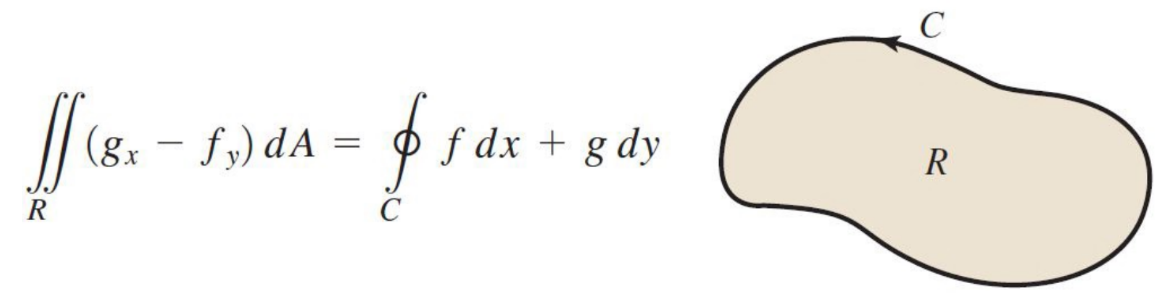
\includegraphics[scale=0.5]{img/imgRGgreen.PNG}
\end{center}

\teorema{\textcolor{red}{Formula de Stokes}}.

\begin{equation}
    \begin{split}
        \begin{array}{c}
            \text{El rotacional del flujo a tráves} \\
            \text{de la superficie cerrada}
        \end{array}
        &=
        \begin{array}{c}
            \text{La integral de un campo vectorial} \\
            \text{sobre una curva cerrada} \ \partial \mathcal{M} 
        \end{array} 
        \\
        \begin{array}{c}
            \displaystyle \iint_{\mathcal{M}} \left(\pdv{B}{x}-\pdv{A}{y}\right)\mathrm{d}x\mathrm{d}y+\iint_{\mathcal{M}} \left(\pdv{C}{y}-\pdv{B}{z}\right)\mathrm{d}y\mathrm{d}z\\
            \displaystyle +\iint_{\mathcal{M}}\left(\pdv{A}{z}-\pdv{C}{x}\right)\mathrm{d}z\mathrm{d}x
        \end{array}
        &=\int_{\partial \mathcal{M}} A\mathrm{d}x+B\mathrm{d}y+C\mathrm{d}z
    \end{split}
\end{equation}

\begin{center}
    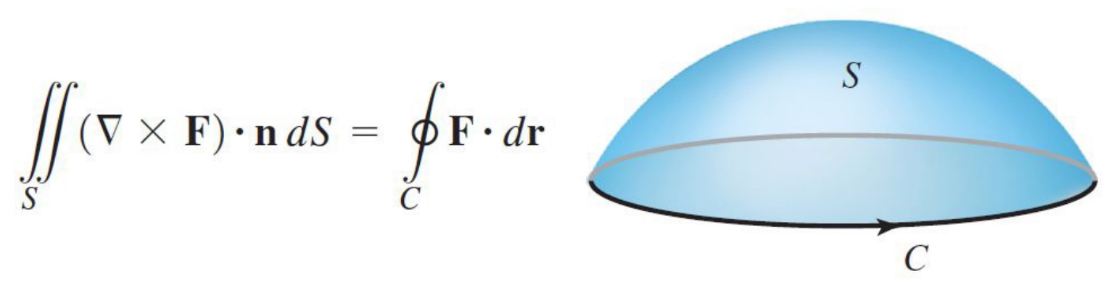
\includegraphics[scale=0.5]{img/imgRGstokes.PNG}
\end{center}

\teorema{\textcolor{red}{Teorema de la Divergencia}}.

\begin{equation}
    \begin{split}
        \begin{array}{c}
            \text{Integral del flujo} \\
            \text{local en el interior}
        \end{array}
        &=
        \begin{array}{c}
            \text{Flujo total hacia afuera a} \\
            \text{través de una superficie} \ S
        \end{array} 
        \\
        \iiint_{\mathcal{M}} \left(\pdv{P}{x}+\pdv{Q}{y}+\pdv{R}{z}\right)\mathrm{d}x\mathrm{d}y\mathrm{d}z&=\iint_{S} P\mathrm{d}y\mathrm{d}z+Q\mathrm{d}z\mathrm{d}x+R\mathrm{d}x\mathrm{d}y
    \end{split}
\end{equation}

\begin{center}
    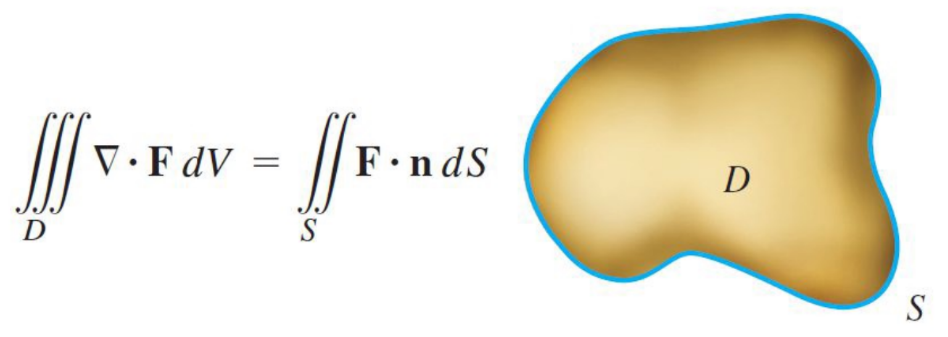
\includegraphics[scale=0.5]{img/imgRGdivergence.PNG}
\end{center}

\teorema{} Si $\mathcal{M}$ es una manifold compacta y orientada sin bordes, entonces para cualquier $\omega \in \Omega^{n-1}(\mathcal{M})$, entonces 
\begin{equation}
    \int_{\mathcal{M}} \mathrm{d}\omega=0.
\end{equation}

\teorema{} Si $\mathcal{M}$ es una variedad compacta orientada en borde, entonces para cualquier $\omega \in \Omega^{n-1}(\mathcal{M})$ con $\mathrm{d}\omega=0$, se tiene 
\begin{equation}
    \int_{\partial \mathcal{M}} \omega=0.
\end{equation}
\section*{Problemas 1}

\begin{enumerate}
    \item \textbf{Manifolds} \\
    En este problema consideraremos varias manifolds utilizando las definiciones usadas en clase:
    \begin{enumerate}[label=(\alph*)]
        \item Considere $\mathbb{R}^n$ en sí mismo como un espacio topológico y construya explícitamente un atlas que muestre que este espacio es una manifold. \textit{Hint:} Una chart es suficiente para la demostración(puede usarse varias charts).
        \item Sean $\mathcal{M}, \mathcal{N}$ dos manifolds suaves y sean los atlas $\{ U_{\alpha}, \phi_{\alpha}\}\{V_{\beta}, \psi_{\beta}\}$ para $\mathcal{M}$ y $\mathcal{N}$ respectivamente. Muestre que el mapa $f: \mathcal{M} \rightarrow \mathcal{N}$ es suave, si para cada $\alpha$ y $\beta$ el mapa $\psi_{\beta} \circ f \circ \psi^{-1}_{\alpha}$ es suave en su dominio de definición.
        \item Muestre que la condición difeomorfismo define una relación de equivalencia para manifolds suaves.
    \end{enumerate}
    \item \textbf{Cálculos en Manifolds} 
    \begin{enumerate}[label=(\alph*)]
        \item Considera $\mathbb{R}^3$ como un manifold con métrica eucilidiana plana y coordenadas $x, y, z$. Introduciremos coordenadas esféricas $r, \theta, \phi$, que están relacionadas con $x, y, z$ mediante
        \begin{equation}
            x=r \sin \theta \cos \phi, \quad y=r \sin \theta \sin \phi, \quad z=r\cos \theta.
        \end{equation}
        Demuestra que la métrica euclidiana plana en coordenadas esféricas tiene la forma
        \begin{equation}
            \mathrm{d}s^2=\mathrm{d}r^2+r^2 \mathrm{d}\theta^2+r^2\sin^2 \theta \mathrm{d}\phi^2
        \end{equation}
        \item Una partícula se mueve a lo largo de una curva parametrizada dada por
        \begin{equation}
            x(\lambda)=\cos \lambda, \quad y(\lambda)=\sin \lambda, \quad z(\lambda)=\lambda
        \end{equation}
        \begin{itemize}
            \item Expresa la trayectoria de la curva en coordenadas polares esféricas $r, \theta, \phi$.
            \item Cálcula los componentes del vector tangente a la curva tanto en los sistemas de coordenadas cartesianas y en polares esféricas.
        \end{itemize}
    \end{enumerate}
    \item \textbf{Lie Bracket} \\
    Considera dos campos $X$ e $Y$, y el conmutador de los vectores, $[X, Y]$, que actúa sobre las funciones $f$ como
    \begin{equation}
        [X, Y]\equiv X(Y(f))-Y(X(f))
    \end{equation}
    \begin{enumerate}[label=(\alph*)]
        \item Demuestra que el producto de los dos campos vectoriales, $XY$, no es un nuevo campo vectorial porque no satisface la regla de Leibniz, y que el conmutador $[X, Y]$ es un nuevo vector dado que sí satisface la regla.
        \item Demuestra que los componentes del Lie Bracket en una base de coordenadas están dados por 
        \begin{equation}
            [X, Y]^{\mu}=X^{\lambda}\partial_{\lambda}Y^{\mu}-Y^{\lambda}\partial_{\lambda}X^{\mu},
        \end{equation}
        y que se cumple que $[Y, X]^{\mu}=-[X, Y]^{\mu}$.
        \item Demuestra explícitamente que $[X, Y]^{\mu}$ transforma como un vector bajo transformaciones de coordenadas.
        \item Confirma que el corchete de Lie obedece la identidad de Jacobi
        \begin{equation}
            [X, [Y, Z]]+[Y, [Z, X]]+[Z, [X, Y]]=0
        \end{equation}
    \end{enumerate}
    \item \textbf{Métrica} \\
    Considera un manifold $\mathcal{M}$ que es 2D, con coordenadas polares ($r, \theta$). El tensor métrico $g$ en $\mathcal{M}$ está dado por:
    \begin{equation}
        g=g_{ij}\mathrm{d}x^{i}\otimes \mathrm{d}x^j=\mathrm{d}r\otimes \mathrm{d}r+r^2\mathrm{d}\theta\otimes\mathrm{d}\theta
    \end{equation}
    donde $g_{ij}$ es una matriz que representa los componentes del tensor métrico.
    \begin{enumerate}[label=(\alph*)]
        \item Verifica las propiedades del tensor métrico $g$:
        \begin{itemize}
            \item $g$ es un campo tensorial suave de tipo ($0, 2$) en $\mathcal{M}$.
            \item $g$ es simétrico. Para cada punto $p$ en el manifold y para cada par de vectores tangentes $u$ y $v$ en $T_p \mathcal{M}$, demuestra que $g_p(u,v)=g_p(v, u)$.
            \item $g$ es no degenerado: Para cada punto $p$ en la variedad y para cada vector tangente $u$ en $T_p\mathcal{M}$, si $g_p(u, v)=0$ para cada $v$ en $T_p\mathcal{M}$, entonces $u=0$. Sugerencia: Considera los vectores tangentes $v=\partial_r$ y $v=\partial_{\theta}$.
        \end{itemize}
    \end{enumerate}
    \item \textbf{Pullback y Métrica inducida}\\
    Considere una manifold $\mathcal{M}$ equipada con una métrica $g$ y una segunda manifold $\mathcal{N}$. Sí además tenemos un mapa diferenciable de la forma $\phi: \mathcal{N}\rightarrow \mathcal{M}$ podemos usar este mapa para ``jalar'' la métrica $g$ hacia $\mathcal{N}$. Esto resulta en lo que es llamado de métrica inducida sobre $\mathcal{N}$, la cual se denota como $\phi^* g$. Con $g$ expandido en coordenadas locales $\{ y^{\mu}\}$ sobre $\mathcal{N}$ la métrica inducida se lee como:
    \begin{equation}
        \phi^* g=\left[g_{\alpha\beta}\left(\pdv{\phi^{\alpha}}{y^{\mu}}\right)\left(\pdv{\phi^{\beta}}{y^{\nu}}\right)\right]\mathrm{d}y^{\mu}\otimes \mathrm{d}y^{\nu}.
    \end{equation}
    Usando estas definiciones considere
    \begin{enumerate}[label=(\alph*)]
        \item Para una dos esfera $S^2$ embebida en $\mathbb{R}^3$, se tiene que:
        \begin{equation}
            S^2=\{R(\cos \phi\sin \theta, \sin \phi\sin \theta, \cos \theta) \ | \ \phi \in [0, 2\pi\rangle, \theta \in [0, \pi\rangle, R>0\}.
        \end{equation}
        Utilice el mapa de inclusión siguiente para el embedding:
        \begin{equation}
            \begin{split}
                S^2 & \Rightarrow \mathbb{R}^3 \\
                (\theta, \phi) & \Rightarrow R(\cos\phi \sin\theta, \sin\phi \sin\theta, \cos\theta)
            \end{split}
        \end{equation}
        para calcular la métrica inducida sobre $S^2$.
        \item En cosmología tendrá importancia el llamado espacio de DeSitter. Este espacio es, fácilmente reconocible por su embedding, como un corte de un espacio de Minkowski 4-dimensional $\mathbb{R}^{1, 4}$ con coordenadas $u, w, x, y, z$ con $u$ siendo la coordenada temporal dada por la ecuación del hiperboloide:
        \begin{equation}
            -u^2+w^2+x^2+y^2+z^2=\alpha^2, \quad \alpha \in \mathbb{R}.
        \end{equation}
        Sobre el espacio DeSitter introducimos las coordenadas $t, \chi, \theta, \phi$ y son inducidas en $\mathbb{R}^{1, 4}$ por:
        \begin{equation}
            \begin{split}
                u&=\alpha \sinh(t/\alpha), \\
                w&=\alpha \cosh(t/\alpha)\cos \chi,\\
                x&=\alpha \cosh(t/\alpha)\sin \chi \cos \theta,\\
                y&=\alpha \cosh(t/\alpha)\sin \chi \sin \theta \cos \phi,\\
                z&=\alpha \cosh(t/\alpha)\sin \chi \sin \theta \sin \phi.
            \end{split}
        \end{equation}
        Calcule la métrica inducida sobre el espacio deSitter.
    \end{enumerate}
\end{enumerate}
\end{adjustwidth}
\end{document}
